
\documentclass[a4paper,titlepage]{scrartcl}
\usepackage[english]{babel}
\usepackage[utf8]{inputenc}
\usepackage[T1]{fontenc}
\usepackage{graphicx}
\usepackage{hyperref}
\usepackage{amsmath,amssymb,amsthm}
\usepackage{siunitx}
\usepackage{booktabs}
\usepackage[format=hang,margin=1cm]{caption}
\usepackage{rotating}
\usepackage{subcaption}
\usepackage{authblk}
\usepackage{color}
\usepackage{xspace}
\usepackage{textgreek}

\begin{document}

%% ----------------------------------------------------------------
%% Definitions.tex
%% ---------------------------------------------------------------- 
\newcommand{\BibTeX}{{\rm B\kern-.05em{\sc i\kern-.025em b}\kern-.08em T\kern-.1667em\lower.7ex\hbox{E}\kern-.125emX}}

%% People
\newcounter{address}
\setcounter{address}{1}
\renewcommand{\theaddress}{\textsuperscript{\fnsymbol{address}}}
\newcommand{\address}[1]{\refstepcounter{address}\theaddress#1\\}
\newcommand{\Name}[3]{\texorpdfstring{\href{mailto:#3}{#2}#1}{#2}\xspace}

%% Abbreviations
\newcommand{\ie}{i.~e.\ }
\newcommand{\eg}{e.~g.\ }
\newcommand{\wrt}{w.~r.~t.\ }
\newcommand{\etal}{\textit{et al.}\xspace}
\newcommand{\Ab}{A\textbeta\xspace}
\newcommand{\Abi}{A\textbeta\textsubscript{1-42}\xspace}
\newcommand{\Abs}{A\textbeta\textsubscript{1-40}\xspace}

%% Maths
\newcommand{\beq}{\begin{equation}}
\newcommand{\eeq}{\end{equation}}
\newcommand{\beqs}{\begin{gather}}
\newcommand{\eeqs}{\end{gather}}
\newcommand{\dd}{\partial}
\newcommand{\vect}[1]{\boldsymbol{#1}}
\newcommand{\velf}{\boldsymbol{u}_f}
\newcommand{\vels}{\boldsymbol{u}_s}
\newcommand{\vareps}{\varepsilon}
\newcommand{\q}{\boldsymbol{q}}
\newcommand{\vel}{\boldsymbol{u}}
\newcommand{\ra}{\rightarrow}
\newcommand{\hatz}{\hat{z}}
\newcommand{\hatt}{\hat{t}}

%% Stress tensor
\newcommand{\taurr}{\tau_{rr}}
\newcommand{\taurt}{\tau_{r\theta}}
\newcommand{\tautt}{\tau_{\theta\theta}}
\newcommand{\tauzz}{\tau_{zz}}
\newcommand{\taurz}{\tau_{rz}}
\newcommand{\taurrl}{\tau_{rr,0}}
\newcommand{\taurtl}{\tau_{r\theta,0}}
\newcommand{\tauttl}{\tau_{\theta\theta,0}}
\newcommand{\tauzzl}{\tau_{zz,0}}
\newcommand{\taurzl}{\tau_{rz,0}}
\newcommand{\taurre}{\tau_{rr,1}}
\newcommand{\taurte}{\tau_{r\theta,1}}
\newcommand{\tautte}{\tau_{\theta\theta,1}}
\newcommand{\tauzze}{\tau_{zz,1}}
\newcommand{\taurze}{\tau_{rz,1}}

%% Strain tensor
\newcommand{\err}{e_{rr}}
\newcommand{\ert}{e_{r\theta}}
\newcommand{\ett}{e_{\theta\theta}}
\newcommand{\ezz}{e_{zz}}
\newcommand{\erz}{e_{rz}}

%% Stress functions
\newcommand{\Airy}{\mathcal{A}}
\newcommand{\Love}{\mathcal{L}}

%% Figures
\newcommand{\onefig}[3]{\begin{figure}\center\includegraphics[width=\linewidth]{#1}\caption{#2}\label{#3}\end{figure}}
\newcommand{\onefighalf}[3]{\begin{figure}\center\includegraphics[width=0.5\linewidth]{#1}\caption{#2}\label{#3}\end{figure}}


\sisetup{range-phrase=--}
\sisetup{range-units=single}

% ----------------------------------------------------------------------------
% Titlepage Parameters
% ----------------------------------------------------------------------------

\title{Arterial pulsations are not powerful enough to drive perivascular drainage of solutes from the brain}
\author[1,2]{Alexandra K. Diem}
\author[2]{Neil W. Bressloff}
\author[3]{Roxana O. Carare}
\author[4]{Giles Richardson}
\affil[1]{Institute for Complex Systems Simulation, University of Southampton, Southampton SO17 1BJ, UK}
\affil[2]{Computational Engineering and Design, Faculty of Engineering \& the Environment, University of Southampton, Southampton SO17 1BJ, UK}
\affil[3]{Faculty of Medicine, University of Southampton, Southampton, UK}
\affil[4]{Faculty of Mathematical Sciences, University of Southampton, Southampton, UK}

\maketitle

\begin{abstract}
\textbf{Summary.} Alzheimer's Disease (AD) is the most common form of dementia and to date there is no preventive medication. Its development is closely related to the accumulation of the neuronal metabolite \Ab, which raises the question of how metabolites are eliminated from the brain. Unlike the rest of the body the brain does not have a lymphatic system and therefore has to eliminate metabolites differently. A connection between the pathology of AD and cerebrovascular diseases has been suggested and confirmed in various mice studies, which has lead to the assumption that interstitial fluid in the basement membranes of cerebral arteries provide the pathways for the perivascular drainage of \Ab. However, perivascular drainage occurs in the reverse direction to arterial blood flow, an effect that lacks an effective explanation. In this study we tested the well-accepted hypothesis that arterial pulsations drive perivascular drainage and additionally that a valve mechanism exists which ensure net reverse drainage. This was examined in terms of a  mathematical model of the  drainage mechanism. It is shown that a valve mechanism (such as directional permeability of the perivascular space) is necessary to achieve a net reverse flow. However, it is also shown that arterial pulsations are not strong enough to produce drainage velocities comparable to experimental observations. % 209 words

Word count: 209

\vspace{1cm}

\textbf{Keywords:} Alzheimer's disease, brain lymphatics, cerebrovascular flow
\end{abstract}


% ----------------------------------------------------------------------------
% Paper Body
% ----------------------------------------------------------------------------

% Introduction

Dementia, a term often used synonymously with Alzheimer's disease (AD), is a symptom of a variety of diseases affecting the human brain and does not constitute a part of normal ageing. Although it has been studied for over 100 years \cite{Selkoe2001}, to date there is no cure as the processes relevant to its onset and progression have not yet been fully understood. The pathology of AD comprises different characteristics, some of which are degeneration and death of neurons, synapse loss, neuroinflammation and the accumulation of waste product deposits \cite{Koffie2011}. The protein amyloid-$\beta$ (\Ab) is produced as part of the normal metabolism of healthy brains, but it plays a major role in the development of AD \cite{Haass1992}. Its accumulation in the walls of cerebral blood vessels as cerebral amyloid angiopathy (CAA) is closely associated with the onset and progression of AD \cite{Weller2006, Weller2009}. CAA strongly correlates with the progression of AD and the degree of dementia as it appears in \SIrange{90}{96}{\percent} of AD patients \cite{Weller2009a}.

In order to process metabolites, the brain requires a lymphatic system that transports waste products to the lymph nodes, where they are decomposed. While the rest of the body possesses a dedicated network of lymphatic vessels these do not exist in the brain \cite{Weller2010}. There is ample evidence that the basement membranes (BM) in the walls of cerebral arteries provide the clearance pathway for interstitial fluid (ISF) towards the surface of the brain, also referred to as perivascular drainage \cite{Weller2010,Carare2008,Hawkes2011,Morris2014}. Because it provides the pathways for perivascular drainage, the BM is also referred to as perivascular space (PVS) in this context. It is important not to confuse this PVS with the Virchow-Robin spaces, which are also often referred to as perivascular (or ``paravascular'') spaces. However, Virchow-Robin spaces are virtual spaces and have no role in \Ab drainage. Additionally, the BM does not actually constitute a space, but rather a fluid-filled protein matrix. Our understanding of the mechanism that drives perivascular drainage through the BM is still very limited. The evidence indicates that ISF enters the BM at the capillary level and flows towards the lymph nodes in the neck via cerebral arteries, but not veins. This suggests that ISF flow is driven in the reverse direction of the blood flow, a phenomenon that does not seem very plausible at first sight \cite{Carare2008}.

A widely accepted hypothesis for the driving mechanism of this reverse perivascular drainage of solutes from the brain is that it is driven by arterial pulsations \cite{Weller2009,Carare2008,Hawkes2011,Morris2014,Schley2006,Attems2011,Wang2011,Iliff2012,Asgari2015,Sharp2015,Weller2015a}. In this paper we tested this hypothesis by using a multi-scale modelling approach combining analytical and numerical methods. The BM is modelled as a porous medium using Darcy's law and a lubrication approximation. Flow inside the BM is driven by both the ISF pressure gradient and the deformation of the arterial wall, which are obtained from a numerical model of the middle cerebral artery (MCA). To guarantee reverse drainage (\ie in the opposite direction of the blood flow) a valve mechanism is implemented as a pressure gradient dependent permeablility. It is shown that this valve mechanism is neccesary to achieve net reverse drainage. The results show that this valve mechanism successfully ensures net reverse drainage inside the BM and is neccesary. However, due to the long wavelength of arterial pulsations the pressure gradients inside the BM were found to be too small to drive fluid flow at the expected velocities. The resulting velocity of the model was approximately two orders of magnitude smaller than values obtained experimentally \cite{Carare2008}. Therefore arterial pulsations are concluded to be insufficient to drive perivascular drainage along the BM of cerebral arteries.


\section{Porous medium model of lymphatic drainage in the BM}
\label{sec:diodemodel}

We propose a model of lymphatic drainage from the brain via the cerebral BM based on Darcy's law for flow in porous media. By exploiting the discrepancy of scales between the width of the BM and its length we approximate the flow by a one-dimensional lubrication model (see for example \cite{Ockendon1995}). Furthermore, we allow the permeability of the BM to depend on the pressure gradient of the ISF. Such a pressure gradient dependent permeability could, for instance, model proteins in the BM protein network that have structural properties that allow them to bend easily only in one direction, thereby acting as a valve, and thus provide a higher resistance to flow in the direction of the blood flow. A similar idea has been investigated in \cite{Sharp2015}, where proteins were explicitly modelled as cillia. However, here we model the active component of the BM generically in this model and thus allow for alternative explanations of the phenomenon.

The BM consists of a complex matrix of proteins (extracellular matrix, ECM) that can be interpreted as a porous medium through which soluble metabolites drain via the ISF. We model flow through this medium, in the standard fashion, by Darcy's law in a 2D cylindrical coordinate system. Darcy's law states that the flux $\q$ is related to the fluid pressure gradient $\boldsymbol{\nabla} p$ by
\beq\label{eq:darcy}
  \q = -K(p_z) \boldsymbol{\nabla} p
\eeq
where $K(p_z)$\footnote{Note that the permeability $K$ used here is the ratio of the intrinsic permeability $k$ of the ECM to the viscosity $\mu$ of ISF, that is $K = k / \mu$} is the pressure gradient dependent permeability of the ECM. We allow the permeability $K$ to be a function of the axial component of the ISF pressure gradient $\partial p(z,t) / \partial z = p_z(z,t)$. In order to obtain a net flux up the vessel, counter to the blood flow, we require this function to be increasing in $p_z$, representing the notion that it is harder to push a flow in the positive $z$-direction ($p_z<0$ and $K(p_z)$ small) than in the negative $z$-direction ($p_z>0$ and $K(p_z)$ large)
\begin{equation}
  K(p_z) = \begin{cases}
    K_0 & p_z > 0\\
    K_1 & p_z \leq 0.
  \end{cases}
\end{equation}

Because of the boundary conditions used we will continue working in terms of the fluid velocity $\vel$, which is related to $\q$ by the linear relationship $\vel = \gamma \, \q$, where $\gamma$ is the porosity of the medium. The governing equations in cylindrical coordinates are thus
\begin{gather}
  u \vect{e_z} + v \vect{e_r} = - \gamma K(p_z) \left( \vect{e_z} p_z + \vect{e_r} p_r \right) \label{eq:darcy_velocity}\\
  u_z + \frac{1}{r} \frac{\dd}{\dd r} \left( r v \right) = 0 \label{eq:continuity},
\end{gather}
where $\vect{e_z}$ and $\vect{e_r}$ describe the unit vectors in the $z$ and $r$ direction. The continuity of velocity is given in \eqref{eq:continuity}.

\begin{figure}
\centerline{\includegraphics{figures/pvs_model.pdf}}
\caption{Geometry of the perivascular drainage pathways model. The length $L$ of a typical artery in the brain can be assumed to be much greater than the width $W$ of the perivascular drainage pathways. Therefore we can approximate the flow as a lubrication model. The pulsation of the capillary is described by the function $h(z,t)$.\label{fig:pvs_model}}
\end{figure}

To determine the boundary conditions of the system consider the geometry in Figure \ref{fig:pvs_model}. Under the assumption that the vessel deformations are radially symmetric the positions of the inner and outer sheaths bounding the BM can be described by the two expressions $r = R_i(z,t)$ and $r = R_o(z,t)$, respectively. Assuming that the flows through the surfaces of the BM are negligible the following kinematic boundary condition applies
\beq \label{eq:kinematic}  
\frac{D}{D t} \left( r - R_i(z,t) \right) = 0 \quad \text{on } r = R_i(z,t)
\eeq
and analogously for $R_o(z,t)$.

Because the BM thickness is much smaller than the vessel length it is possible, on using the lubrication approximation, to derive a 1D model (in $z$) for the BM thickness $h(z,t)$; this takes the form
\beq
\frac{\dd}{\dd t} \left( R_i(z,t) \cdot h(z,t) \right) = \frac{\dd}{\dd z} \left( R_i(z,t) \cdot h(z,t) \cdot K(p_{z}) \cdot p_{z} \right),\label{eq:pvs_model}
\eeq
which describes the evolution of the BM thickness and can be solved using a finite difference approximation. Consider an infinitesimally small volume of BM $dV = 2\pi \cdot R_i(z,t) \cdot h(z,t) \cdot dz$. Then the difference between the flux into and out of the element $dV$ is equal to $\dd (dV)/ \dd t$, which can be written as
\begin{align}
2\pi \frac{\dd}{\dd t} \left( R_i(z,t) \cdot h(z,t) \right) &= \nonumber \\ 
2\pi \cdot R_i(z,t) \cdot h(z,t) & \cdot q(z,t) - 2\pi \cdot R_i(z + dz,t) \cdot h(z + dz,t) \cdot q(z + dz,t),
\end{align}
which is equal to the model equation \eqref{eq:pvs_model}. For a detailed derivation see Supplementary Information 1. The pressure $p(z,t)$ and the displacement of the BM wall $R_i(z,t)$ are, to a very good approximation, determined solely by the arterial pressure (\ie almost independent of the BM flow), see Supplementary Information 2 for more details. $R_i(z,t)$ and $p_z$ can be obtained from a numerical artery model described in the next section.


\section{Numerical Model of a Straight Arterial Section}

\begin{table}
\center
\caption{Parameters used to simulate the MCA including the first bifurcation.\label{tab:parameter}}
\begin{tabular}{ccc}
\toprule
Parameter & Value & Physical meaning\\
\midrule
\multicolumn{3}{l}{MCA}\\
\midrule
$R_u$ & \SI{0.14}{\centi\metre} & upstream radius\\
$R_d$ & \SI{0.14}{\centi\metre} & downstream radius\\
$L$ & \SI{7}{\centi\metre} & length\\
\midrule
\multicolumn{3}{l}{Left daughter vessel}\\
\midrule
$R_u$ & \SI{0.13}{\centi\metre} & upstream radius\\
$R_d$ & \SI{0.08}{\centi\metre} & downstream radius\\
$L$ & \SI{6.5}{\centi\metre} & length\\
\midrule
\multicolumn{3}{l}{Right daughter vessel}\\
\midrule
$R_u$ & \SI{0.13}{\centi\metre} & upstream radius\\
$R_d$ & \SI{0.08}{\centi\metre} & downstream radius\\
$L$ & \SI{6.4}{\centi\metre} & length\\
\midrule
\multicolumn{3}{l}{Simulation parameters}\\
\midrule
$k_1$ & \SI{2.0e7}{\gram\per\centi\metre\per\square\second} & wall elasticity parameter (see \cite{Olufsen2000,Diem2016a})\\
$k_2$ & \SI{-22.53}{\per\centi\metre} & wall elasticity parameter (see \cite{Olufsen2000,Diem2016a})\\
$k_3$ & \SI{8.65e5}{\gram\per\centi\metre\per\square\second} & wall elasticity parameter (see \cite{Olufsen2000,Diem2016a})\\
$R_1$ & \SI{14130}{\gram\per\centi\metre\tothe{4}\per\second} & First resistance element\\
$R_2$ & \SI{7200}{\gram\per\centi\metre\tothe{4}\per\second} & Second resistance element\\
$C_T$ & \SI{2.4752e-3}{\centi\metre\tothe{4}\square\second\per\gram} & Compliance element\\
$T$ & \SI{0.85}{\second} & cardiac cycle length\\
$t_c$ & 4 & number of cardiac cycles simulated\\
$\Delta t$ & \SI{1e-5}{\second} & time step size\\
$\Delta z$ & \SI{0.1}{\centi\metre} & spatial step size\\
\bottomrule
\end{tabular}
\end{table}

Following the geometry outlined in \autoref{sec:diodemodel} arteries are modelled as axisymmetric tubes in a cylindrical coordinate system with cross-sectional area $A(z,t) = \pi R(z,t)^2$ and flux $q(z,t)$. Following the derivations in \cite{Olufsen2000,Diem2016} arteries are represented by the conservation law
\begin{equation}
  \frac{\dd \boldsymbol{U}}{\dd t} + \frac{\dd \boldsymbol{F}}{\dd z} = \boldsymbol{S}, \label{eq:conservation}
\end{equation}
where
\begin{gather*}
  \boldsymbol{U} = \begin{pmatrix} A(z,t) \\ q(z,t) \end{pmatrix}, \quad \boldsymbol{F} = \begin{pmatrix} q(z,t)\\ \dfrac{q(z,t)^2}{A(z,t)} + f(r_0) \sqrt{A_0(z) A(z,t)} \end{pmatrix}, \quad \boldsymbol{S} = \begin{pmatrix} 0\\ S_1 \end{pmatrix}\\
  \begin{split}
    S_1 = -&\frac{2 \pi R(z,t)}{\delta_b \mathrm{Re}} \frac{q(z,t)}{A(z,t)} +\\
    &\left( 2 \sqrt{A(z,t)} \left( \sqrt{\pi} f(r_0) + \sqrt{A_0(z)} \frac{df(r_0)}{dr_0 } \right) - A(z,t) \frac{df(r_0)}{dr_0} \right) \frac{dr_0(z)}{dz}.
  \end{split}
\end{gather*}
This system of equations can be solved numerically using Richtmyer's two-step version of the Lax-Wendroff method, as done by others \cite{Olufsen2000,LeVeque1992,Kolachalama2007}. We use the code from \cite{Diem2016a}, which is an implementation of the Lax-Wendroff method in Python, to implement a model of the MCA and its first bifurcation. All simulation parameters are listed in \autoref{tab:parameter}. The MCA radius was taken from \cite{Cousins2014} and following their estimate that generally the length of an artery is $50 \cdot R_u$ lengths were calculated accordingly. The radii of the daughter vessels were estimated using a scaling factor of 0.91, also obtained from \cite{Cousins2014}. The length of the right daughter vessel was shortened slightly to avoid reflective waves cancelling one another out, as also done in \cite{Kolachalama2007}. A three-element Windkessel (3WK) model is used at the outlet whose parameters were obtained from \cite{Olufsen2002}.

\begin{figure}
\centerline{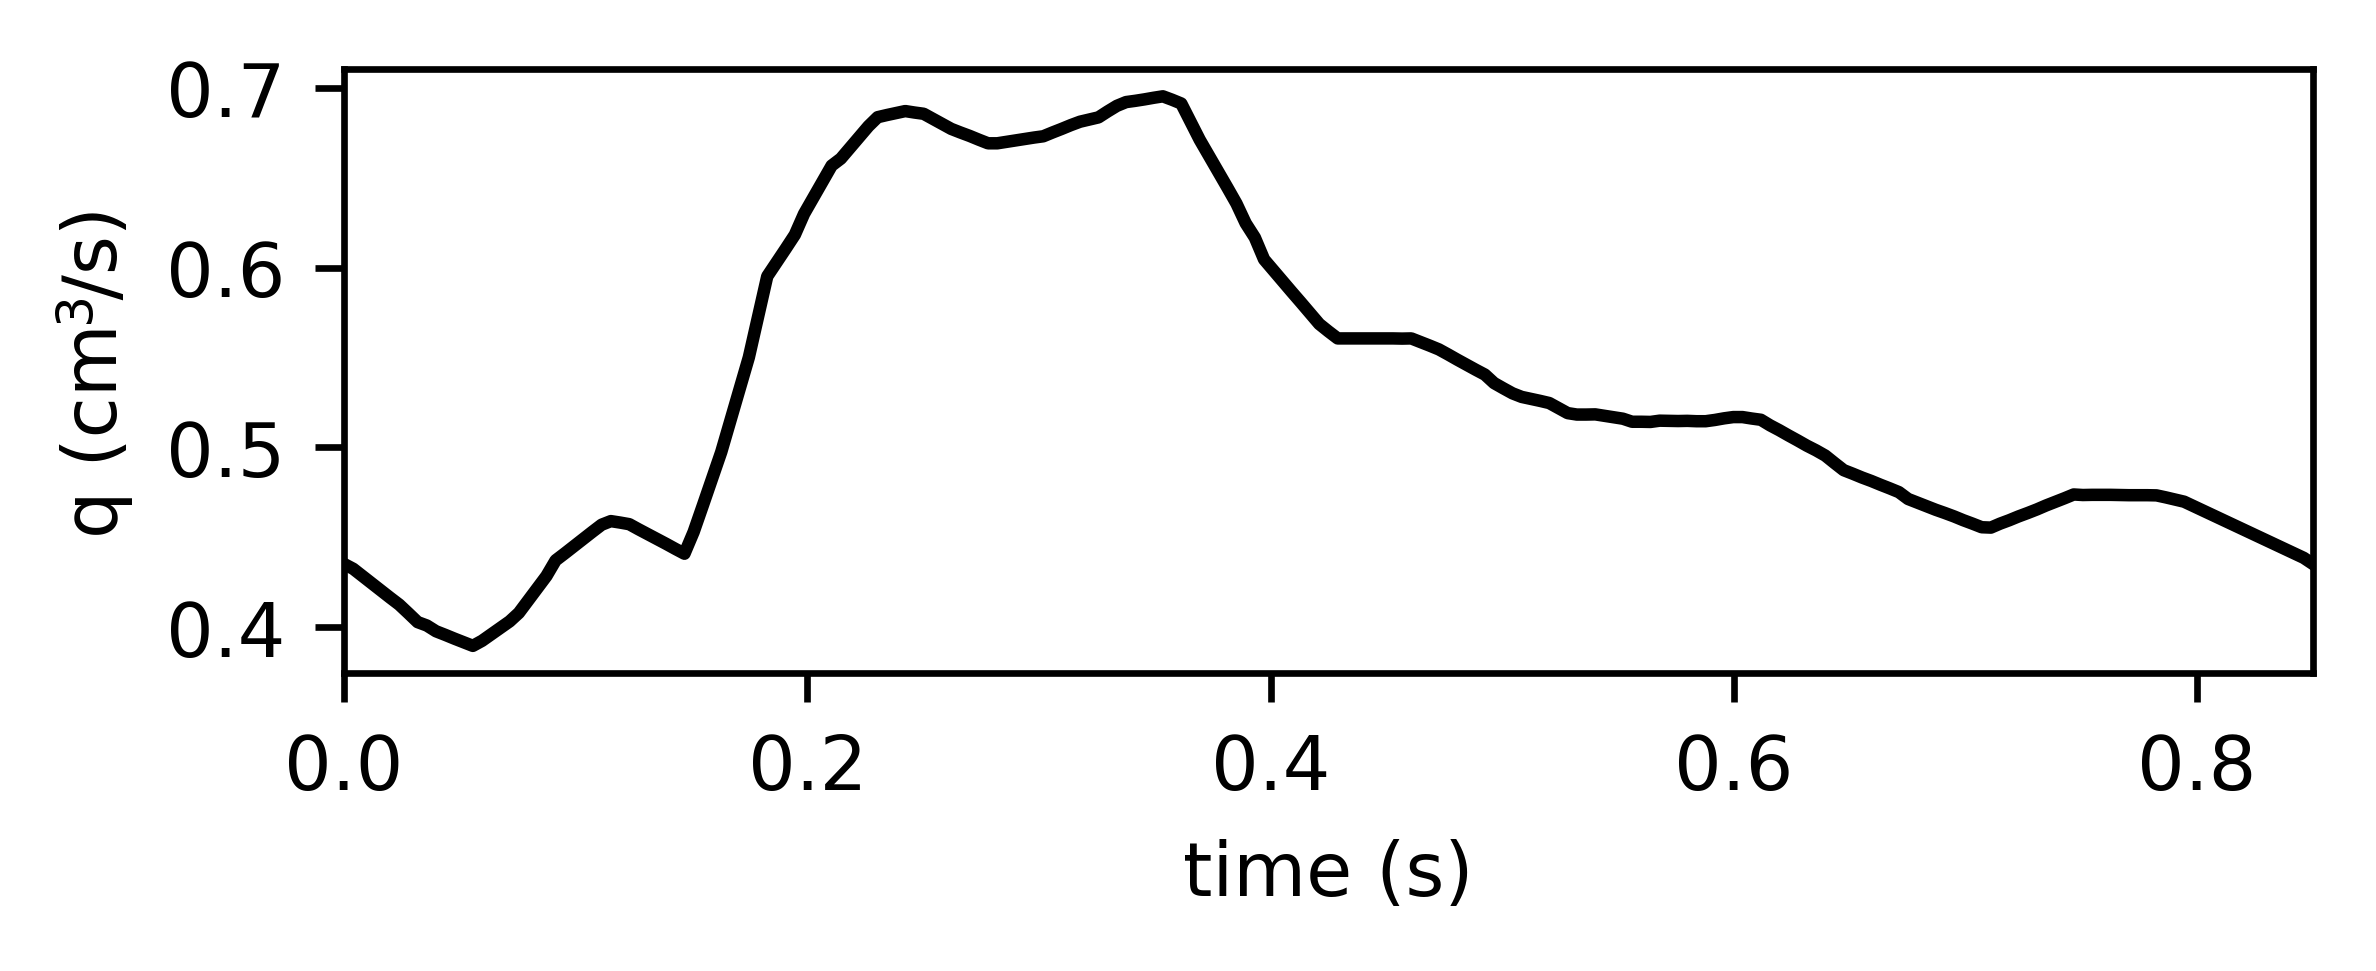
\includegraphics{figures/inlet.png}}
\caption{Inlet function for MCA simulations obtained from patient-specific measurements. The final ten peaks of the velocity time series were averaged in the Fourier space and adjusted such that its range of values aligns with those reported in \cite{Olufsen2002}. The resulting inlet function is smooth and serves as the inlet boundary condition for the MCA simulations using VaMpy \cite{Diem2016a}.\label{fig:inlet}}
\end{figure}

At the inlet flux is prescribed directly. Patient-specific flow velocity measurements were collected from the MCA of a healthy adult male using Doppler Sonography ultrasound. The velocity data was adjusted to obtain volumetric flux values within the range reported in \cite{Olufsen2002}. To obtain a smooth inlet function the final ten peaks of the time series were averaged in the Fourier space. The resulting inlet boundary condition is shown in \autoref{fig:inlet}.

\begin{figure}
\centerline{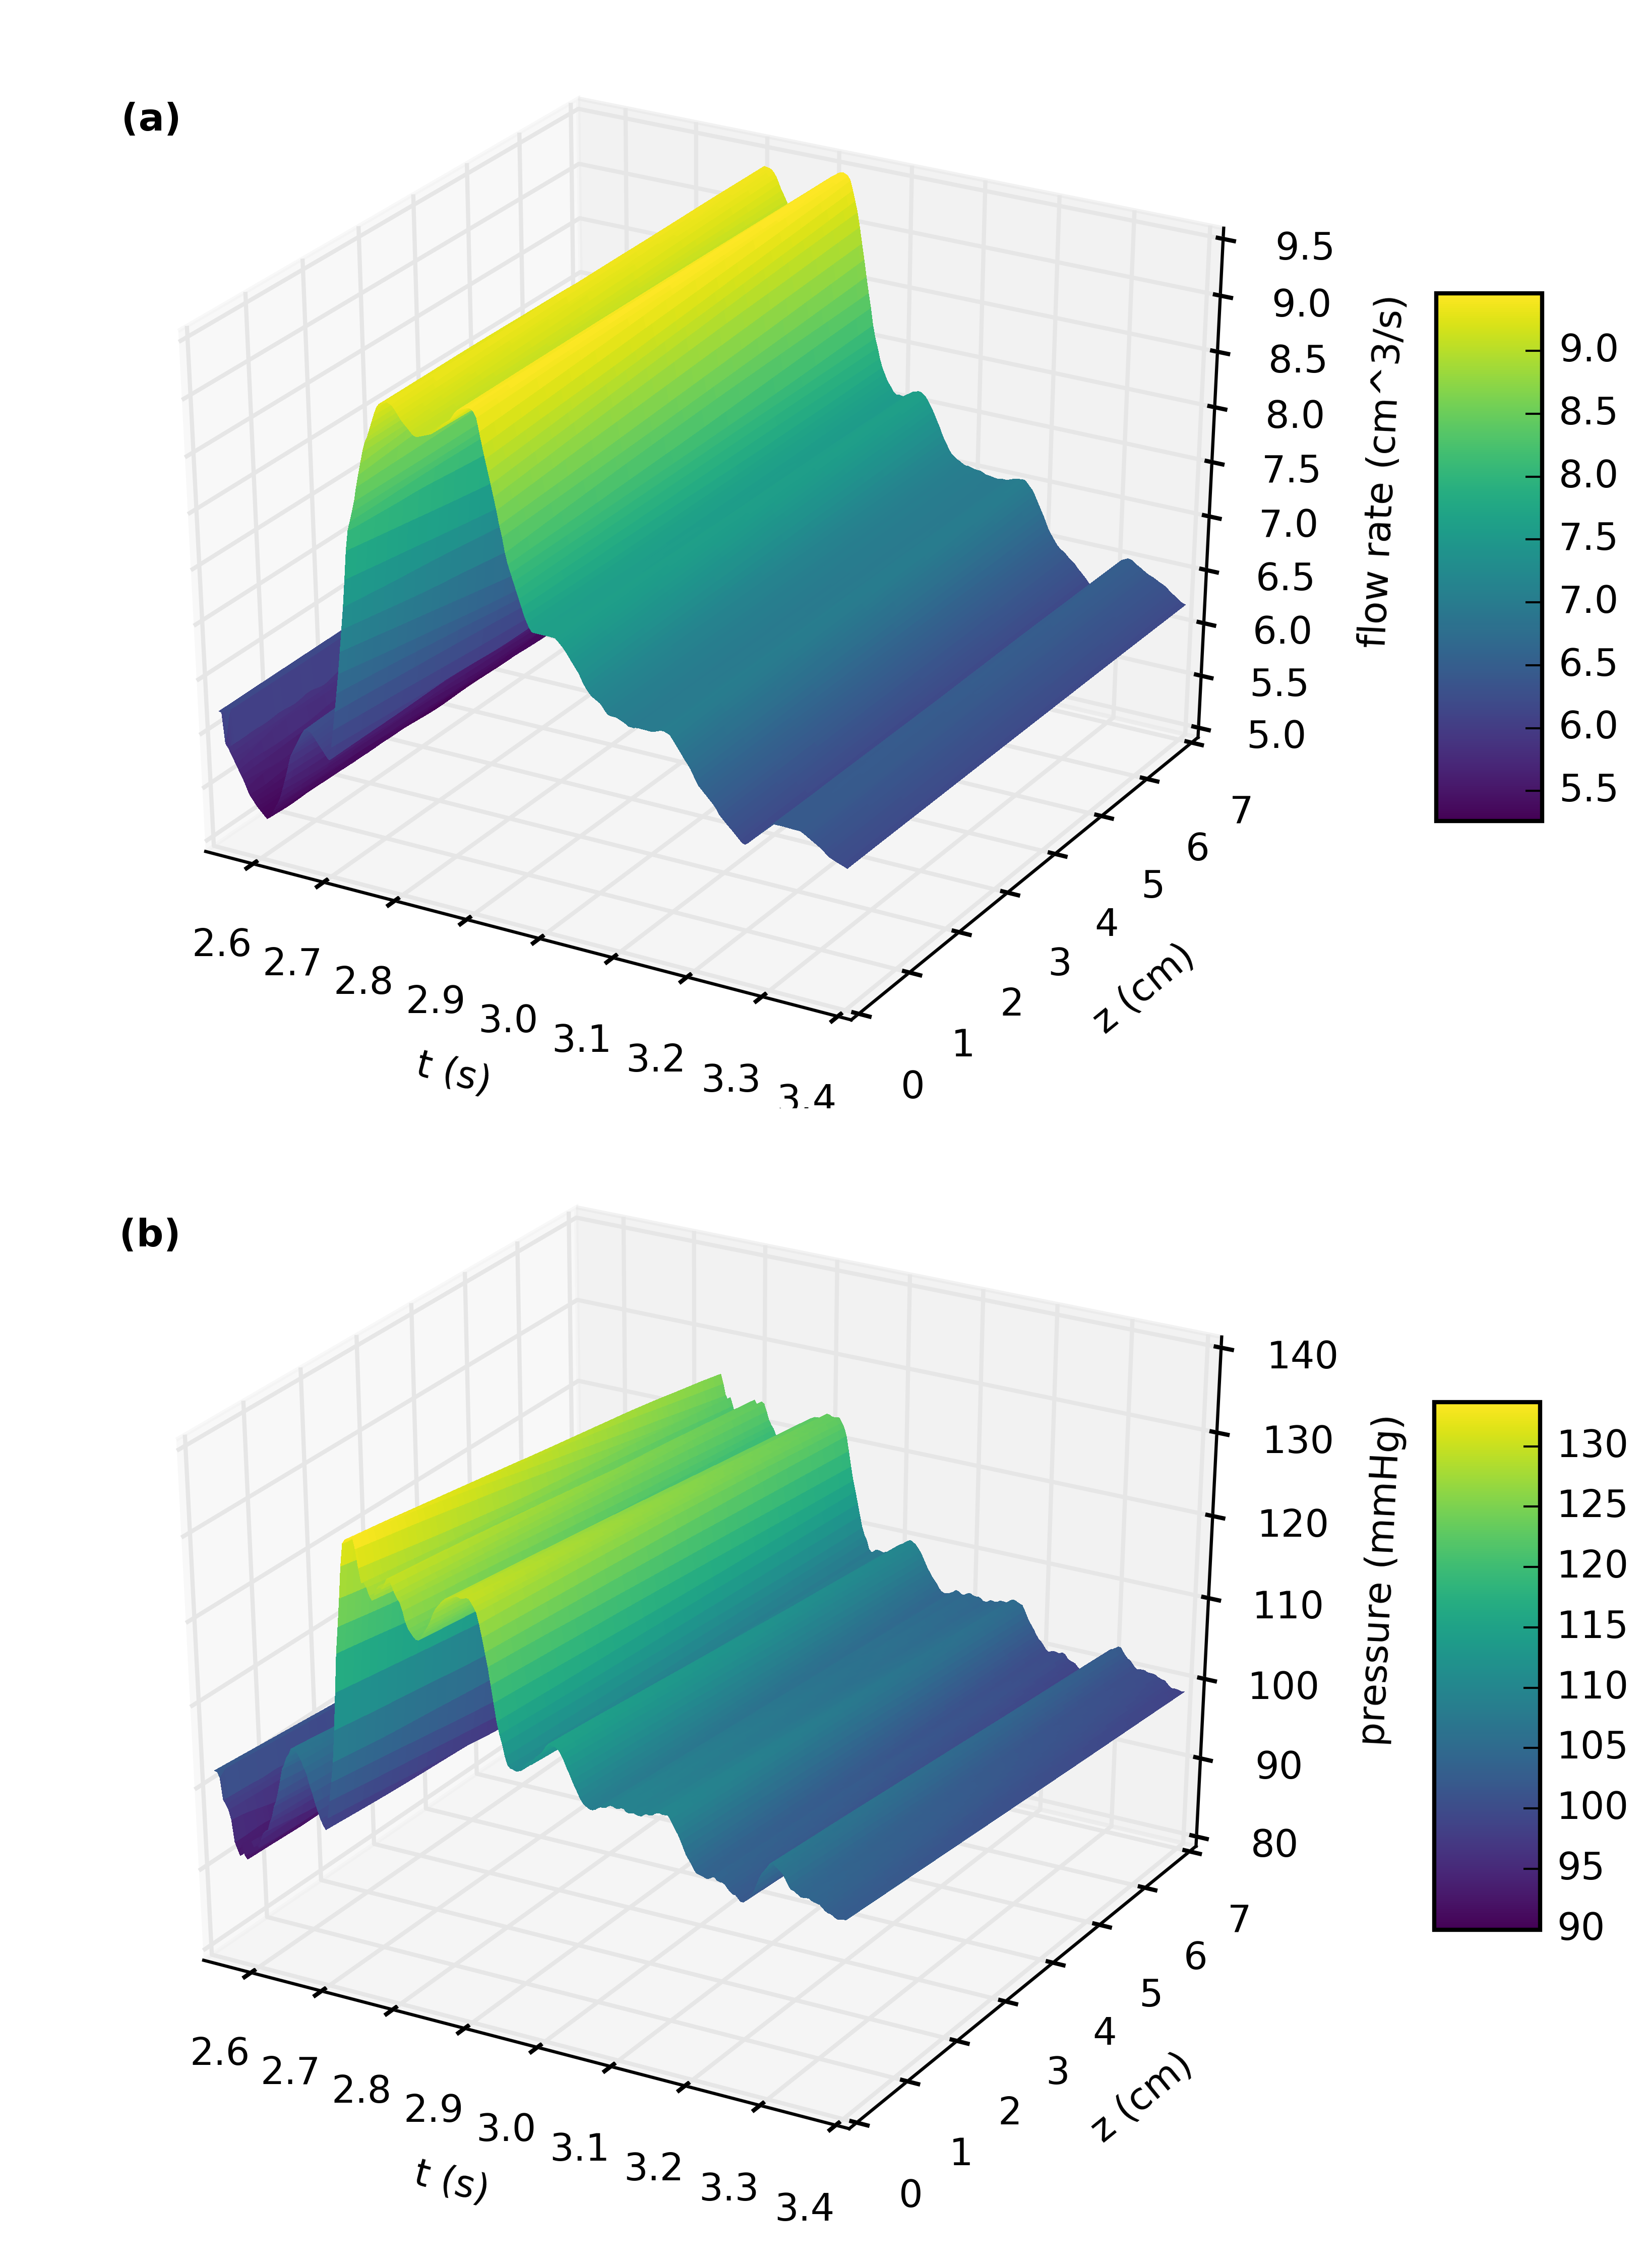
\includegraphics{figures/mca.png}}
\caption{Flux (a) and pressure (b) in the MCA. Simulations were performed using the VaMpy Python package \cite{Diem2016a} and the simulation parameters are listed in \autoref{tab:parameter}. Wall stiffness is high in small blood vessels, therefore pressure gradients in time are steep.\label{fig:mca}}
\end{figure}

MCA simulations were run for four cardiac cycles to allow the system to settle. \autoref{fig:mca} shows flow and pressure in the MCA. Because the radius of the MCA is very small its wall stiffness is high. Pressure gradients in time are therefore steep. This data provides the basis for estimating perivascular drainage through the cerebral vasculature.


\section{Perivascular Drainage through the MCA}

In the previous sections the models governing blood flow through the MCA and ISF flow through the artery wall have been introduced. Here, the results of the previous sections are coupled and used to calculate ISF flow through the BM with and without a valve mechanism to show its necessity to achieve net reverse drainage. At the same time it is shown that blood pressure driven perivascular drainage is far too slow to provide any meaningful flow, thereby disproving the popular hypothesis that arterial pulsations provide the major driving force for perivascular drainage.

\begin{figure}
\centerline{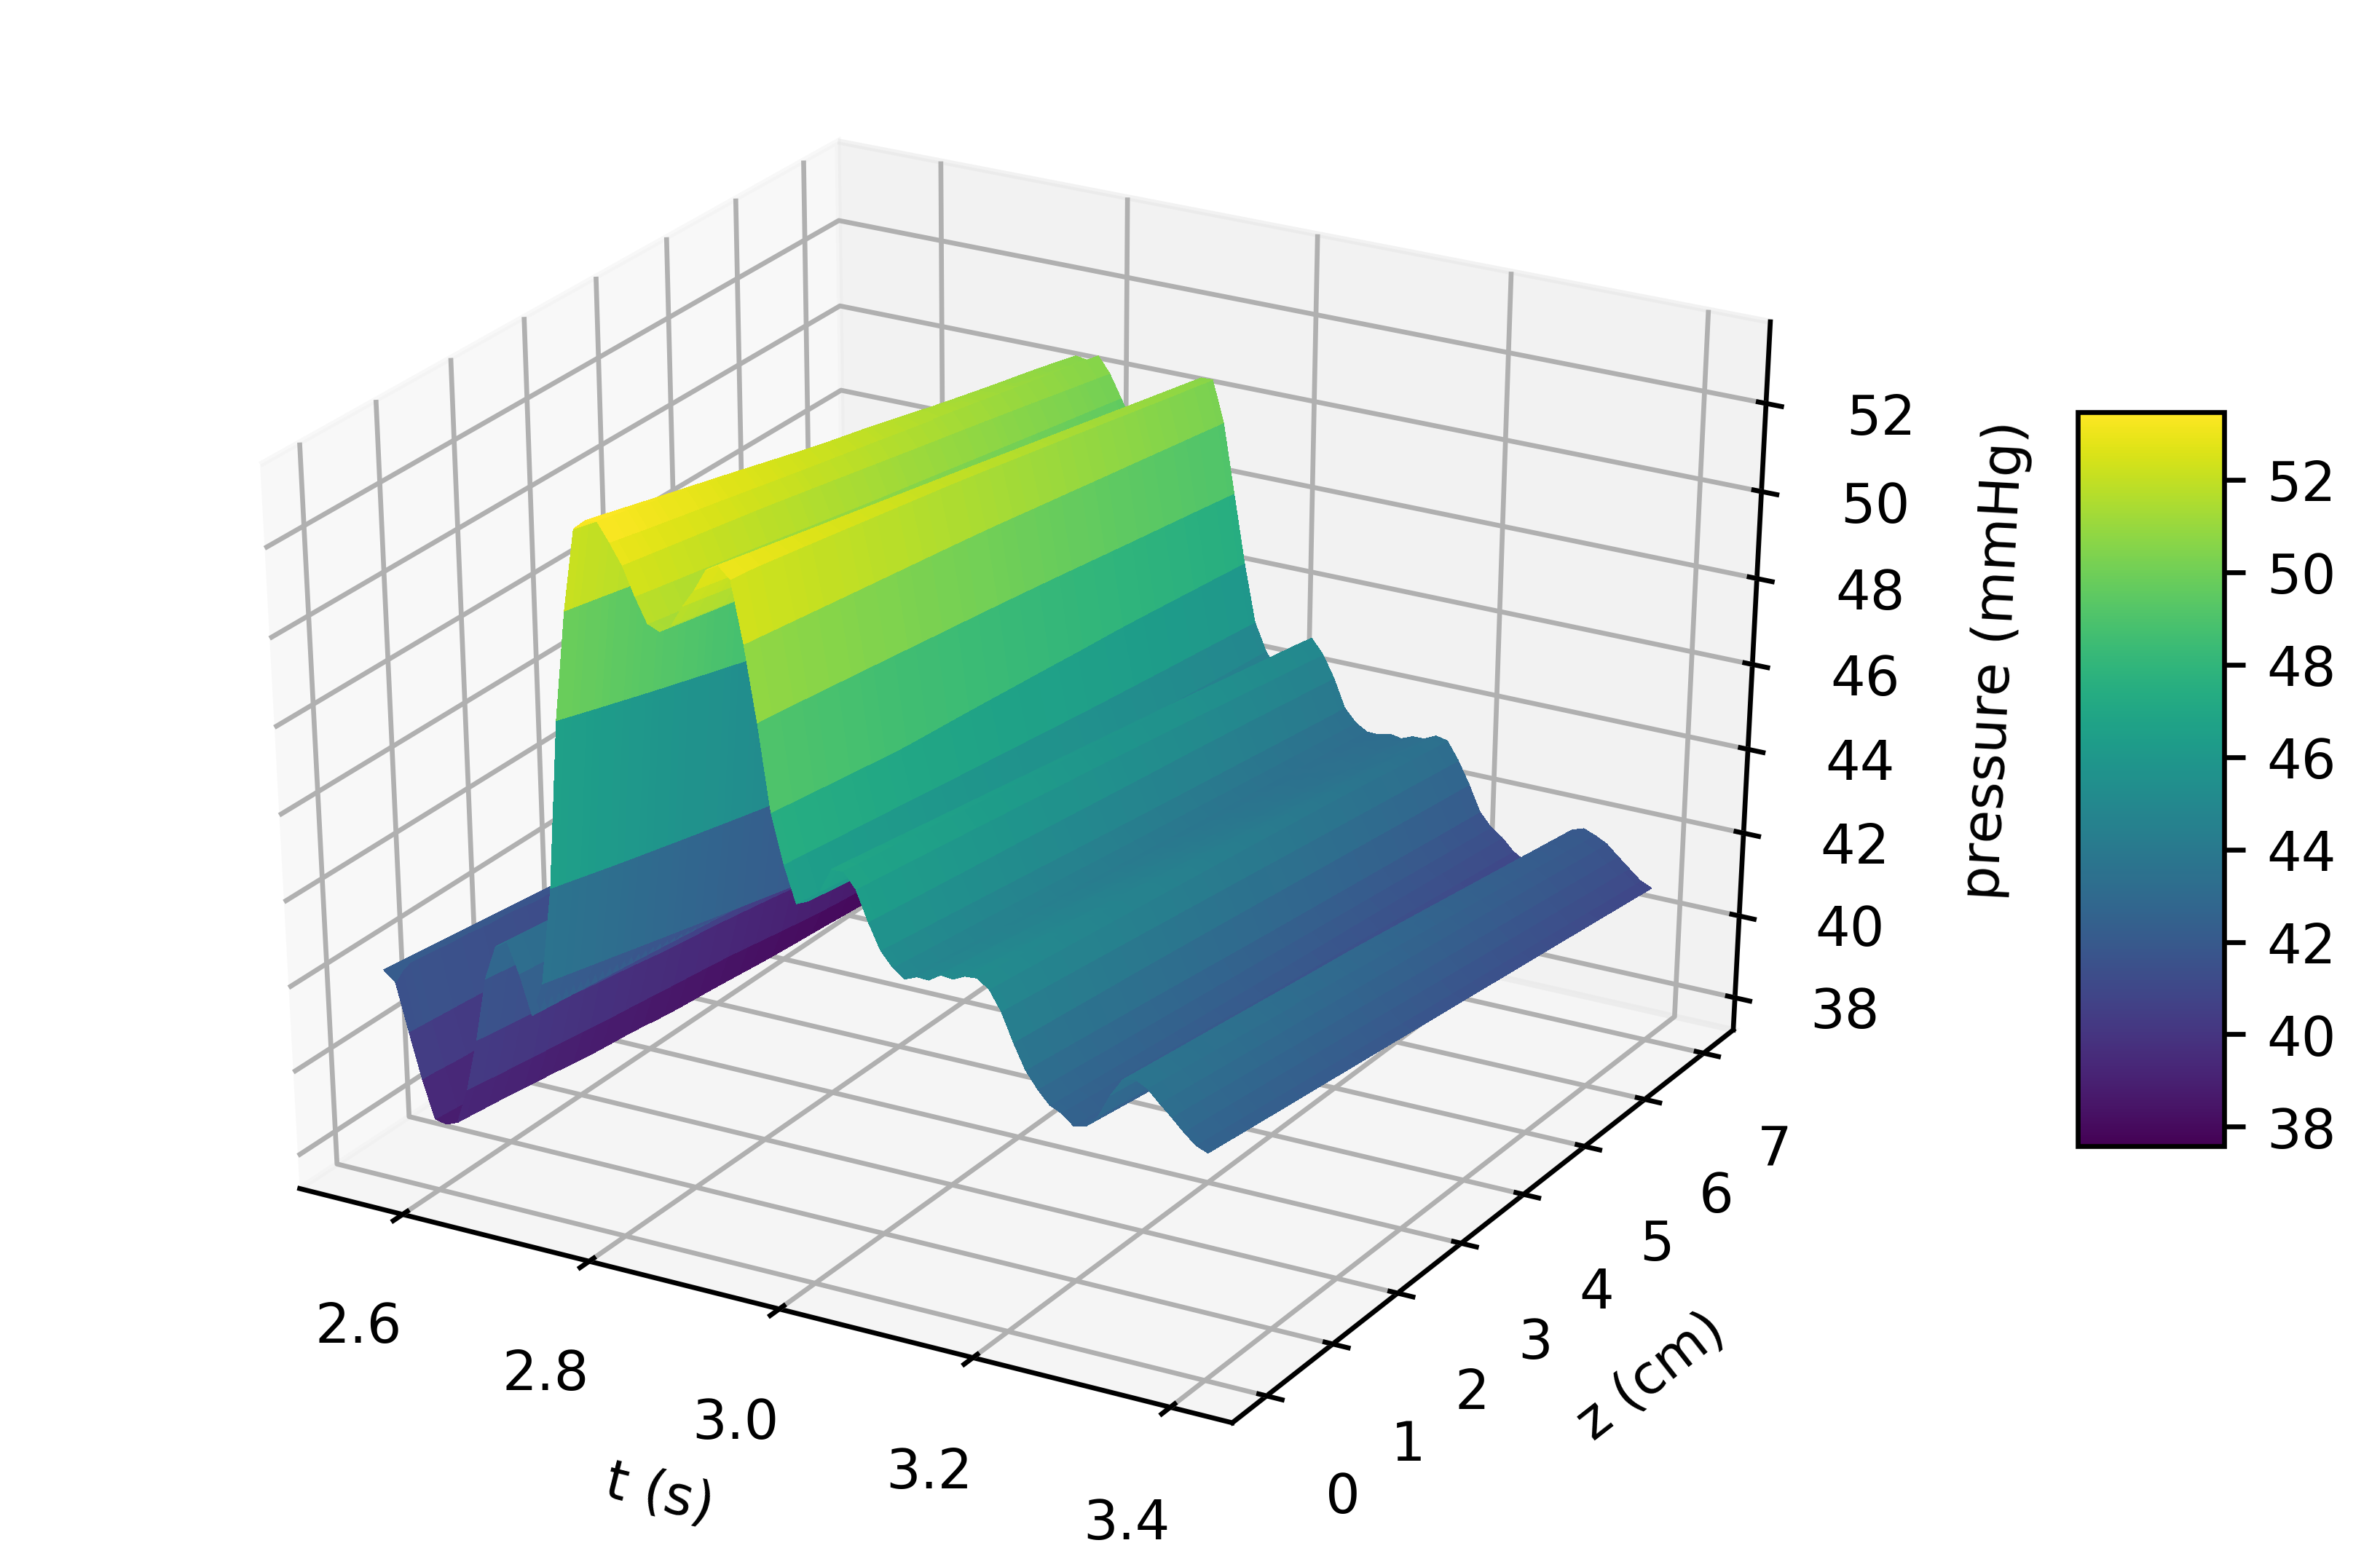
\includegraphics{figures/bm_pressure.png}}
\caption{ISF pressure inside the BM of the MCA. To obtain ISF pressure the radial stresses inside the wall were calculated from the blood pressure inside the artery. ISF pressure is directly proportional to the radial stress in the wall at the location of the BM (see Supplementary Information 2). Flow velocity was then calculated using Darcy's law.\label{fig:bm_pressure}}
\end{figure}

\begin{figure}
\centerline{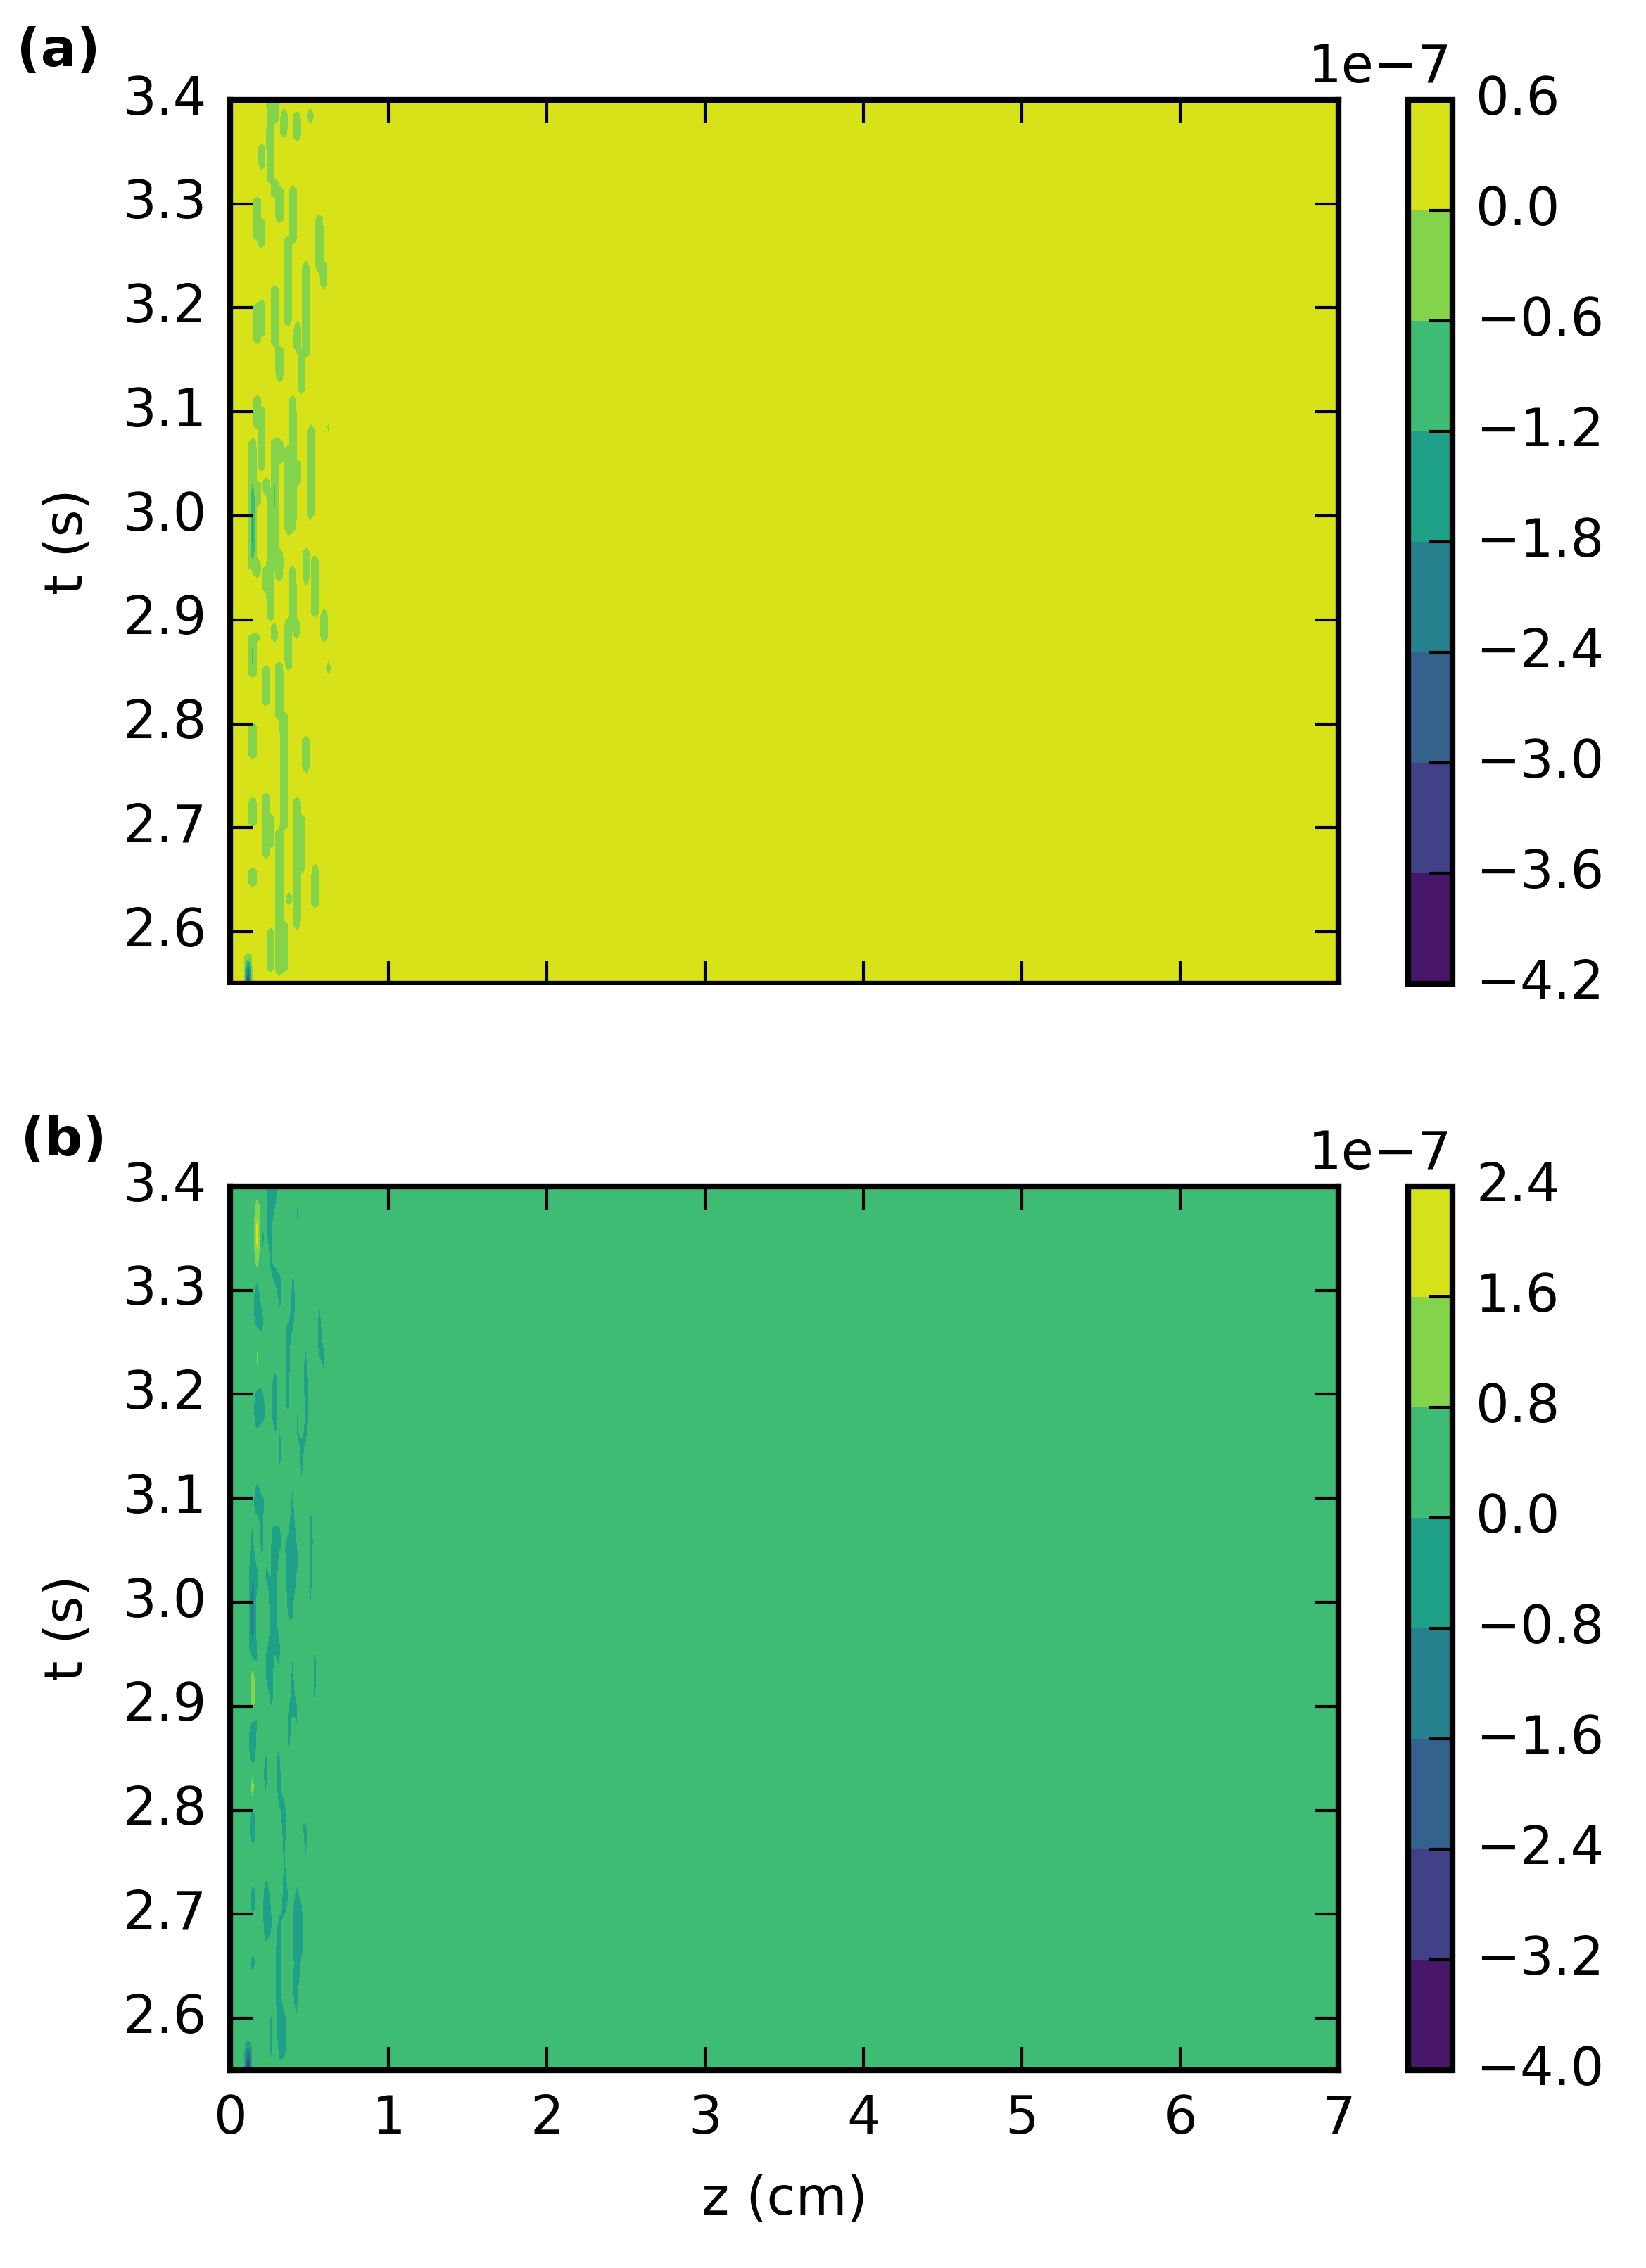
\includegraphics{figures/bm_velocity.png}}
\caption{ISF velocity inside the BM of the MCA with (a) and without a valve mechanism (b) at $r = r_0 + 0.5h$. The average flow velocity with a valve mechanism is \SI{-3.54e-6}{\micro\metre\per\second} ($K_0/K_1$ = 0.01), while without a valve mechanism it is \SI{7.91e-4}{\micro\metre\per\second}. A negative value indicates net reverse flow, confirming that a valve mechanism is required to drive flow in the reverse direction of the blood. The expected magnitude of drainage is \SI{8.33}{\micro\metre\per\second} \cite{Carare2008}.\label{fig:bm_velocity}}
\end{figure}

ISF pressure inside the BM (at $r = r_0 + 0.5h$) is shown in \autoref{fig:bm_pressure}. Velocity wth and without a valve mechanism are shown in \autoref{fig:bm_velocity}. The results show that a valve mechanism is required to drive perivascular drainage in the reverse direction of the blood flow with an average flow velocity of \SI{-3.54e-6}{\micro\metre\per\second} for a ratio of $K_0/K_1 = 0.01$, while it is \SI{7.91e-4}{\micro\metre\per\second}. While the results confirm the necessity of a strong valve mechanism under pulse driven flow they also indicate that arterial pulsations are not strong enough to drive perivascular drainage. Drainage velocity is fastest without a valve mechanism (and then it is in the wrong direction), but even in that case it is four orders of magnitude slower than the expected value of \SI{8.33}{\micro\metre\per\second} \cite{Carare2008}. The valve mechanism only guarantees net reverse drainage for a permeability ratio $K_0/K_1 < 1.6e-2$.

\begin{figure}
\centerline{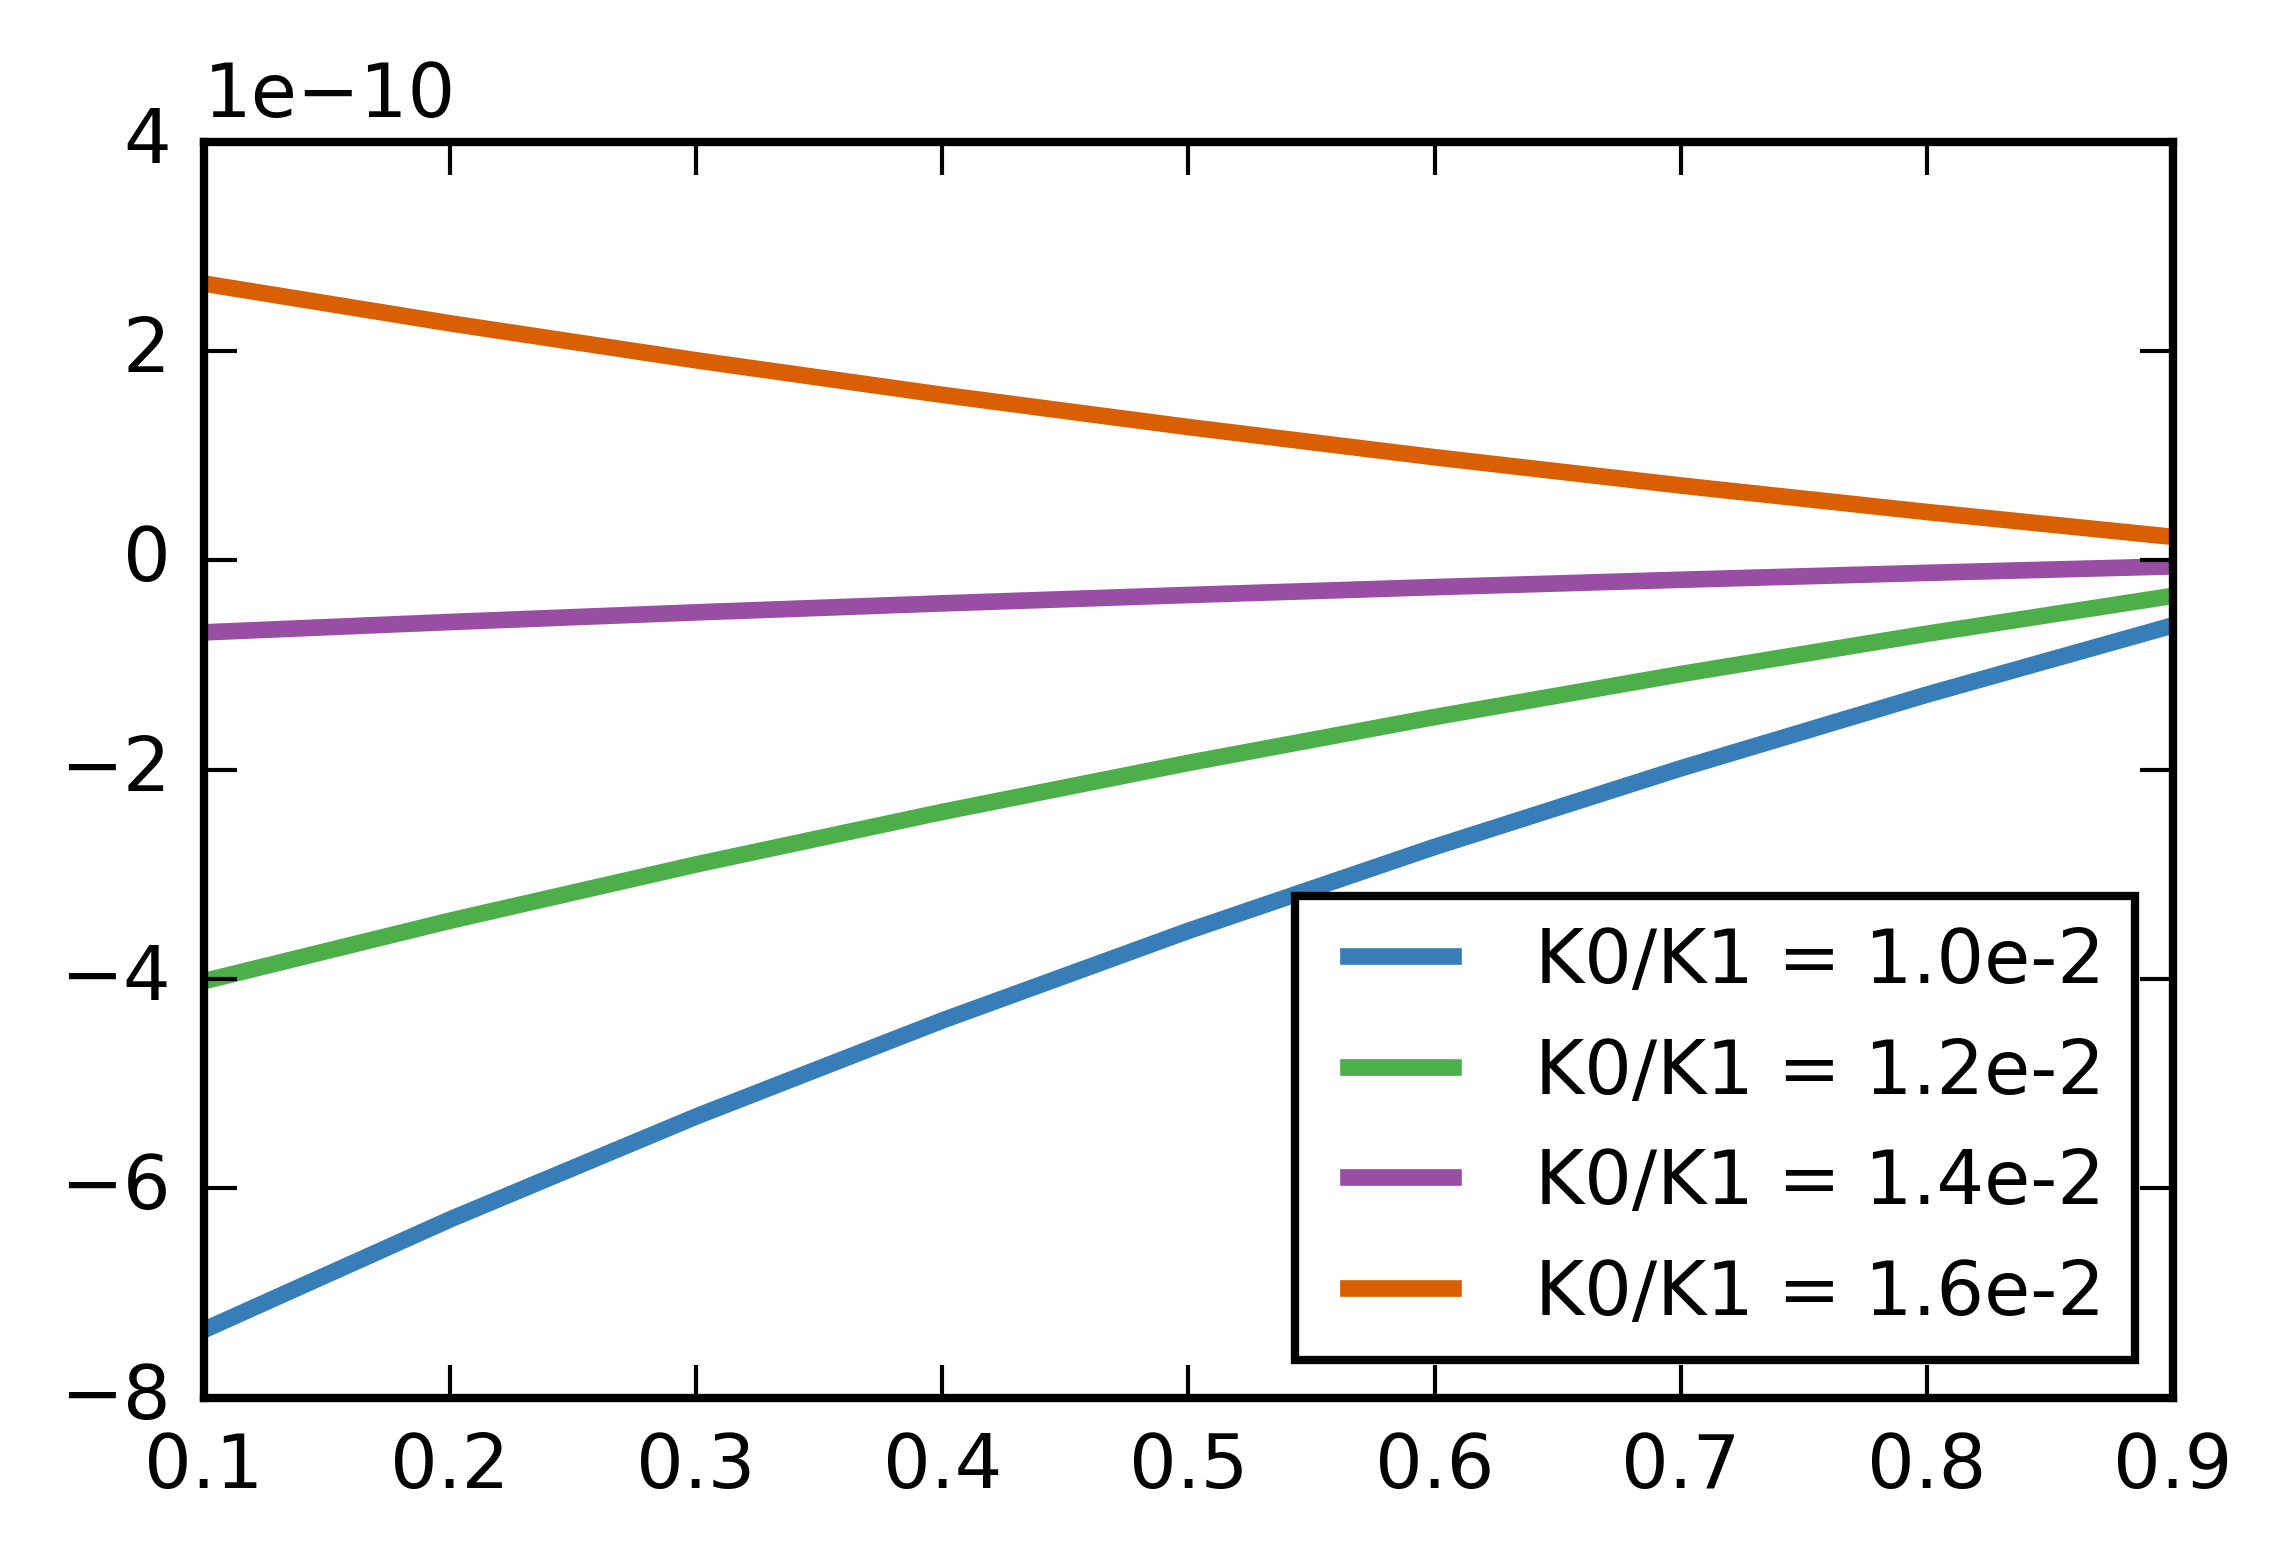
\includegraphics{figures/valve_test.png}}
\caption{ISF velocity at $r = r_0 + xh$. Drainage occurs in the reverse direction of the blood flow for $K_0/K_1 = \SI{1.6e-2}{}$ and is fastest at $r = r_0 + 0.1h$. The fastest net reverse drainage is \SI{-7.35e-6}{\micro\metre\per\second}, which is six orders of magnitude smaller than the expected value of \SI{-8.33}{\micro\metre\per\second}.\label{fig:valve_test}}
\end{figure}


\section{Discussion and Conclusion}

The results show that the valve mechanism as implemented in our analytical model of the BM guarantees net reverse flow inside the BM under physiological blood flow conditions. The valve mechanism is required to be strong, \ie the ratio of $K_0/K_1$ needs to be small. Additionally, the model shows that a valve mechanism is neccessary for net reverse flow to occur within the BM, confirming results from previous studies that did not include a valve mechanism and concluded the existence of some attachment mechanism \cite{Schley2006,Wang2011}. Net drainage additionally depends on the distance of the BM from the artery lumen. The closer the BM is placed to the lumen the faster net reverse drainage is, but variations remain within the same order of magnitude. This is due to the relatively large thickness of cerebral artery walls and their elastic properties. The hypothesis that the BM utilises a unidirectional valve mechanism is plausible as the general lymphatic system of the body also has one and its existence has previously been speculated \cite{Weller2010,Schley2006,Heppell2013}.

Since the development of the Schley model we have gained knowledge on the approximate velocity of the drainage and are able to perform imaging in live mice \cite{Carare2008,Schley2006,Arbel-Ornath2013}, yet this key information has not been utilised in more recent mathematical and computational studies \cite{Wang2011,Sharp2015}. From the results of Carare et al. \cite{Carare2008} it was estimated that the velocity for perivascular drainage in blood vessels of roughly \SI{10}{\micro\metre} in diameter is in the order of magnitude of \SI{8}{\micro\metre\per\second}. Arbel-Ornath et~al. \cite{Arbel-Ornath2013} measured the dye intensity of the tracers, which does not allow them to directly measure the velocity of the drainage but, from their results, a half-life period of about five minutes can be assumed for their \SI{3}{\micro\litre} injection volume. Therefore, we would expect a volumetric flux in the order of magnitude of \SI{0.001}{\cubic\milli\metre\per\second}. No correlation between ISF velocity and artery diameter was found.

The results from this study showed that the average drainage velocity of ISF is \SI{-3.54e-6}{\micro\metre\per\second} at $r = r_0 + 0.5h$ and $K_0/K_1 = 0.01$. This value indicates a net reverse flow within the BM, although it is six orders of magnitude smaller than what would be expected \cite{Carare2008}. The results therefore suggest that arterial pulsations are not powerful enough to drive perivascular drainage of ISF through the BM. This is most likely due to the very long wavelength of the arterial pulsations compared to the artery section considered, which results in very small pressure gradients along the vessel length (\autoref{fig:mca}b). It appears that other forces are neccessary to produce the pressure gradients required to push fluid through the BM and an interesting candidate for such forces is vasomotion of smooth muscle cells \cite{DiMarco2015}.

In conclusion, this study indicates that under physiological conditions arterial pulsations alone are too weak to drive perivascular drainage of ISF through the arterial BM. This result is especially interesting as arterial pulsations have been treated as the most likely candidate for the driving force of perivascular drainage. Other studies, which have considered arterial pulsations as driving mechanisms have either concluded that ISF flow in the reverse direction to the blood flow requires some form of attachment mechanism \cite{Schley2006,Wang2011} or require very specific protein movements giving rise to valve-like behaviour \cite{Sharp2015}. Our model is the first to suggest a very general valve mechanism that reliably produces net reverse drainage along the BM. While the valve model of the BM provides a phyisologically feasible mechanism to ensure net reverse drainage of ISF it is insufficient to drive the physiologically observed flow (by several orders of magnitude). This result is therefore significant as it disproves the widely accepted arterial pulsation hypothesis of perivascular drainage of \Ab from the brain \cite{Weller2009,Carare2008,Hawkes2011,Morris2014,Schley2006,Attems2011,Wang2011,Iliff2012,Asgari2015,Sharp2015,Weller2015a} and suggests that other forces have to be considered instead.

% ----------------------------------------------------------------------------
% Acknowledgements
% ----------------------------------------------------------------------------
\section*{Acknowledgements}

This work was supported by an EPSRC Doctoral Training Centre grant (EP/G03690X/1) and EPSRC Doctoral Training Partnership grant (EP/N509747/1). The authors thank Tony Birch for carrying out the middle cerebral artery flow velocity measurements and Roy O. Weller for his continued advice and encouragement.

% ----------------------------------------------------------------------------
% Appendix
% ----------------------------------------------------------------------------
%\section*{Appendix}
%\appendix
%\input{mathanalysis}
%\input{airystress}

% ----------------------------------------------------------------------------
% References
% ----------------------------------------------------------------------------
\addcontentsline{toc}{section}{\bibname}

\begin{thebibliography}{10}
\bibitem{Selkoe2001}
Selkoe~DJ (2001) Alzheimer's Disease: Genes, Proteins and Therapies. {\em Physiol.~Rev.} 81(2):741--766.

\bibitem{Koffie2011}
Koffie~RM, Hyman~BT and Spires-Jones~TL (2011) Alzheimer's disease: synapses gone cold. {\em Mol.~Neurodegener.} 21(1):63.

\bibitem{Haass1992}
Haass~C et~al. (1992) Amyloid $\beta$-peptide is produced by cultured cells during normal metabolism. {\em Nature} 359(6393):322--325.

\bibitem{Weller2006}
Weller~RO, Massey~A, Kuo~YM and Roher~AE (2006) Cerebral amyloid angiopathy: accumulation of A$\beta$ in interstitial fluid drainage pathways in Alzheimer's disease. {\em Ann.~N.~Y.~Acad.~Sci.} 903(1):110--117.

\bibitem{Weller2009}
Weller~RO, Carare~RO and Boche~D (2009) Amyloid: Vascular and Parenchymal. {\em Encyclpedia of Neuroscience}, ed Squire~LR (Oxford Academic Press), pp.~355--362.

\bibitem{Weller2009a}
Weller~RO, Preston~SD, Subash~M and Carare~RO (2009) Cerebral amyloid angiopathy in the aetiology and immunotherapy of Alzheimer's disease. {\em Alzheimer's~Res.~Ther.} 1(2):6.

\bibitem{Weller2010}
Weller~RO, Galea~I, Carare~RO and Minagar~A (2010) Pathophysiology of the lymphatic drainage system of the central nervous system: Implication for pathogenesis and therapy of multiple sclerosis. {\em Pathophysiology} 17(4):295--306.

\bibitem{Carare2008}
Carare~RO et~al. (2008) Solutes, but not cells, drain from the brain parenchyma along basement membranes of capillaries and arteries: significance for cerebral amyloid angiopathy and neuroimmunology. {\em Neuropathol.~Appl.~Neurobiol.} 34(2):131--144.

\bibitem{Hawkes2011}
Hawkes~CA et~al. (2011) Perivascular drainage of solutes is impaired in the ageing mouse brain and in the presence of cerebral amyloid angiopathy. {\em Acta~Neuropathol.} 121(4):431--443.

\bibitem{Morris2014}
Morris~AWJ, Carare~RO, Schreiber~S and Hawkes~CA (2014) The cerebrovascular basement membrane: role in the clearance of $\beta$-amyloid and cerebral amyloid angiopathy. {\em Front.~Aging~Neurosci.} 6:251.

\bibitem{Schley2006}
Schley~D, Carare-Nnadi~R, Please~CP, Perry~VH and Weller~RO (2006) Mechanisms to explain the reverse perivascular transport of solutes out of the brain. {\em J.~Theor.~Biol.} 238(4):962--974.

\bibitem{Attems2011}
Attems~J, Jellinger~K, Thal~DR and Van~Nostrand~W (2011) Review: Sporadic cerebral amyloid angiopathy. {\em Neuropathol.~Appl.~Neurobiol.} 37(1):75--93.

\bibitem{Wang2011}
Wang~P and Olbricht~WL (2011) Fluid mechanics in the perivascular space. {\em J.~Theor.~Biol.} 247(1): 52--57.

\bibitem{Iliff2012}
Iliff~JJ et~al. (2012) A Paravascular Pathway Facilitates CSF Flow Through the Brain Parenchyma and the Clearance of Interstitial Solutes, Including Amyloid $\beta$. {\em Sci.~Transl.~Med.} 4(147):147ra111.

\bibitem{Asgari2015}
Asgari~M, De~Z\'elicourt~D and Kurtcuoglu~V (2015) How astrocyte networks may contribute to cerebral metabolite clearance. {\em Sci.~Rep.} 5:15024.

\bibitem{Sharp2015}
Sharp~MK, Diem~AK, Weller~RO, Carare~RO (2015) Peristalsis with Oscillating Flow Resistance: A Mechanism for Periarterial Clearance of Amyloid Beta from the Brain. {\em Ann.~Biomed.~Eng.} doi~10.1007/s10439-015-1457-6.

\bibitem{Weller2015a}
Weller~RO, Hawkes~CA, Kalaria~RN, Werring~DJ, Carare~RO (2015) White Matter Changes in Dementia: Role of Impaired Drainage of Interstitial Fluid. {\em Brain~Pathol.} 25(1):63--78.

\bibitem{Ockendon1995}
Ockendon~H and Ockendon~JR (1995) Viscous Flow, Cambridge University Press, Cambridge, UK.

\bibitem{Olufsen2000}
Olufsen~MS et~al. (2000) Numerical Simulation and Experimental Validation of Blood Flow in Arteries with Structured-Tree Outflow Conditions. {\em Ann.~Biomed.~Eng.} 28(11):1281--1299.

\bibitem{Diem2016}
Diem~AK (2016) Prediction of Perivascular Drainage of \Ab from the Brain Using Compuational Modelling: Implication for Alzheimer's Disease. {\em PhD~Thesis.}

\bibitem{LeVeque1992}
LeVeque~RJ (1992) Numerical Methods for Conservation Laws, Birkh\"auser Verlag, Basel, Switzerland.

\bibitem{Kolachalama2007}
Kolachalama~V, Bressloff~NW, Nair~PB, Shearman~CP (2007) Predictive Haemodynamics in a One-Dimensional Carotid Artery Bifurcation. Part I: Application to Stent Design. {\em IEEE~Trans.~Biomed.~Eng.} 54(5):802--812.

\bibitem{Diem2016a}
Diem~AK, Bressloff~NW (2016) VaMpy: A Python Package to Solve 1D Blood Flow Problems. {\em JORS.} Submitted.

\bibitem{Cousins2014}
Cousins~W, Gremaud~PA (2014) Impedance boundary conditions for general transient hemodynamics. {\em Int.~J.~Numer.~Method~Biomed.~Eng.}
  
\bibitem{Olufsen2002}
Olufsen~MS, Nadim~A, Lipsitz~LA (2002) Dynamics of cerebral blood flow regulation explained using a lumped parameter model. {\em Am.~J.~Physiol.~Regul.~Integr.~Comp.~Physiol.} 282(2):R611--R622.



\bibitem{Heppell2013}
Heppell~C, Richarson~G and Roose~T (2013) A Model for Fluid Drainage by the Lymphatic System. {\em Bull.~Math.~Biol.} 75(1):49--81.

\bibitem{Arbel-Ornath2013}
Arbel-Ornath~M et~al. (2013) Interstitial fluid drainage is impaired in ischemic stroke and Alzheimer's disease mouse models. {\em Acta~Neuropathol.} 126(3):353--364.

\bibitem{DiMarco2015}
Di~Marco~LY, Farkas~E, Martin~C, Venneri~A and Frangi~AF (2015) Is Vasomotion in Cerebral Arteries Impaired in Alzheimer's Disease? {\em J.~Alzheimers~Dis.} 46(1):35--53.
\end{thebibliography}


\end{document}

